\documentclass[12pt, twoside]{article}
\usepackage[letterpaper, margin=1in, headsep=0.5in]{geometry}
\usepackage[english]{babel}
\usepackage[utf8]{inputenc}
\usepackage{amsmath}
\usepackage{amsfonts}
\usepackage{amssymb}
\usepackage{tikz}
\usetikzlibrary{quotes, angles}
\usepackage{graphicx}
\usepackage{enumitem}
\usepackage{multicol}

\newif\ifmeta
\metatrue %print standards and topics tags

\title{Regents Geometry}
\author{Chris Huson}
\date{September 2020}

\usepackage{fancyhdr}
\pagestyle{fancy}
\fancyhf{}
\renewcommand{\headrulewidth}{0pt} % disable the underline of the header
\raggedbottom


\fancyhead[LE]{\thepage}
\fancyhead[RO]{\thepage \\ Name: \hspace{4cm} \,\\}
\fancyhead[LO]{BECA / Dr. Huson / Geometry 08-Area+volume\\* pset ID: 124}

\begin{document}

\subsubsection*{8-11CW-Tank-volume}
\begin{enumerate}
\item A water tank is in the shape of a cylinder with a hemispherical bottom and conical top. The diameter of the tank is 6 feet, and the height of the cylindrical body is 8 feet, as shown in the diagram. \\[0.25cm]
  If water fills the tank to the top of the cylinder (but not into the cone), find the volume of water it holds. Round your answer to the nearest whole cubic foot.
  \begin{flushright}
  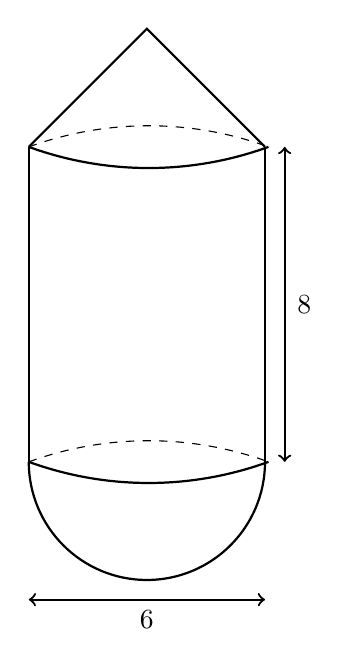
\begin{tikzpicture}[scale=.5]
    %\draw [help lines] (-2,-4) grid (8,12);
    %\draw [thick, ->] (-2.2,0) -- (8.4,0) node [below right] {$x$};
    %\draw [thick, ->] (0,-1.2)--(0,7.4) node [left] {$y$};
    \draw [thick] (0,0)--(0,8);
    \draw [thick] (6,0)--(6,8);
    \draw [thick] (0,8)--(3,11)--(6,8);
    \draw [thick] (0,0) arc (180:360:3);
    \draw [thick] (0,0) arc (-110:-70:8.9);
    \draw [dashed] (0,0) arc (110:70:8.9);
    \draw [thick] (0,8) arc (-110:-70:8.9);
    \draw [dashed] (0,8) arc (110:70:8.9);
    \draw [thick, <->] (6.5,0)--(6.5,8);
    \node at (7,4){$8$};
    \draw [thick, <->] (0,-3.5)--(6,-3.5);
    \node at (3,-4){$6$};
  \end{tikzpicture}
\end{flushright} %\vspace{1cm}

\item A water tank is in the shape of a cylinder with a hemispherical bottom and conical top. Overall, the tank stands 26 feet tall with a diameter of 10 feet. The conical top is 6 feet tall. \\[0.25cm]
  Find the volume of the tank to top of the cylinder (not including the cone). Round your answer to the nearest tenth of a cubic foot.
  \begin{flushright}
  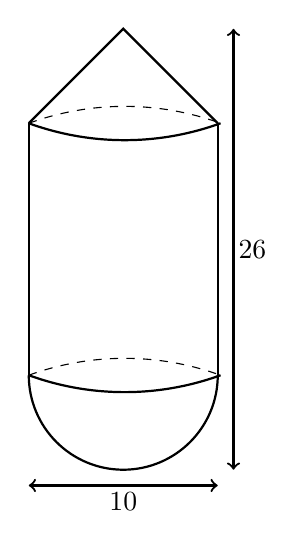
\begin{tikzpicture}[scale=.4]
    %\draw [help lines] (-2,-4) grid (8,12);
    %\draw [thick, ->] (-2.2,0) -- (8.4,0) node [below right] {$x$};
    %\draw [thick, ->] (0,-1.2)--(0,7.4) node [left] {$y$};
    \draw [thick] (0,0)--(0,8);
    \draw [thick] (6,0)--(6,8);
    \draw [thick] (0,8)--(3,11)--(6,8);
    \draw [thick] (0,0) arc (180:360:3);
    \draw [thick] (0,0) arc (-110:-70:8.9);
    \draw [dashed] (0,0) arc (110:70:8.9);
    \draw [thick] (0,8) arc (-110:-70:8.9);
    \draw [dashed] (0,8) arc (110:70:8.9);
    \draw [thick, <->] (6.5,-3)--(6.5,11);
    \node at (7.1,4){$26$};
    \draw [thick, <->] (0,-3.5)--(6,-3.5);
    \node at (3,-4){$10$};
  \end{tikzpicture}
\end{flushright}

\newpage
\item A backyard swimming pool has the shape of a cylinder 12 feet in diameter and 4 feet high, as shown in the diagram.
  \begin{enumerate}
    \item If the water comes up to 6 inches below the top of the pool, find the volume of water it holds. Round your answer to the nearest whole cubic foot.
    \begin{flushright}
    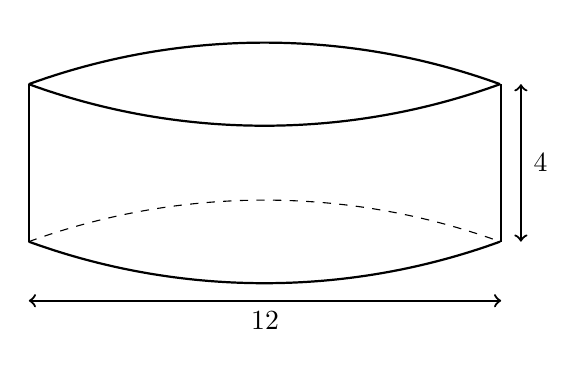
\begin{tikzpicture}[scale=.5]
      %\draw [help lines] (-2,-4) grid (8,12);
      %\draw [thick, ->] (-2.2,0) -- (8.4,0) node [below right] {$x$};
      %\draw [thick, ->] (0,-1.2)--(0,7.4) node [left] {$y$};
      \draw [thick] (0,0)--(0,4);
      \draw [thick] (12,0)--(12,4);
      %\draw [thick] (0,8)--(3,11)--(6,8);
      %\draw [thick] (0,0) arc (180:360:3);
      \draw [thick] (0,0) arc (-110:-70:17.5);
      \draw [dashed] (0,0) arc (110:70:17.5);
      \draw [thick] (0,4) arc (-110:-70:17.5);
      \draw [thick] (0,4) arc (110:70:17.5);
      \draw [thick, <->] (12.5,0)--(12.5,4);
      \node at (13,2){$4$};
      \draw [thick, <->] (0,-1.5)--(12,-1.5);
      \node at (6,-2){$12$};
    \end{tikzpicture}
  \end{flushright} \vspace{2cm}
  \item Find the volume in gallons of water. There are 7.5 gallons per cubic foot. \vspace{4cm}
  \item The owner decides to drain the pool using a small pump with a capacity of 3 gallons per minute. Can the pump empty the pool in less than 24 hours?
\end{enumerate}

\end{enumerate}
\end{document}